\documentclass[10pt,a4paper]{article}

% =========================================================================
% Packages
% =========================================================================
\usepackage[utf8]{inputenc}
\usepackage[T1]{fontenc}
\usepackage{lmodern}
\usepackage{geometry}
\usepackage{graphicx}
\graphicspath{{Gambar/}}
\usepackage{amsmath,amssymb}
\usepackage{fancyhdr}
\usepackage{titlesec}
\usepackage{booktabs}
\usepackage{tabularx}
\usepackage{array}
\usepackage{caption}
\usepackage{subcaption}
\usepackage{algorithm}
\usepackage{algpseudocode}
\usepackage{hyperref}
\usepackage{microtype}
\usepackage{url}
\usepackage{cite}

% =========================================================================
% Page Geometry & Margins
% Format: A4 Paper, Margins: Top, Bottom, Left, Right = 2.5 cm
% =========================================================================
\geometry{
  a4paper,
  top=2.5cm,
  bottom=2.5cm,
  left=2.5cm,
  right=2.5cm,
  headheight=45pt,
  headsep=12pt,
  footskip=24pt
}

% Paragraph settings: Justified, single space, no paragraph indent
\setlength{\parindent}{0pt}
\setlength{\parskip}{6pt}
\linespread{1.0}

% Hyperlink configuration
\hypersetup{
  colorlinks=true,
  linkcolor=blue,
  citecolor=blue,
  urlcolor=blue
}

% =========================================================================
% Header & Footer Settings
% =========================================================================
\pagestyle{fancy}
\fancyhf{}
\fancyhead[L]{\fontsize{9pt}{11pt}\selectfont JURNAL TEKNOLOGI REKAYASA INFORMASI DAN KOMPUTER}
\fancyfoot[R]{\fontsize{9pt}{11pt}\selectfont\thepage}
\renewcommand{\headrulewidth}{0.4pt}
\renewcommand{\footrulewidth}{0pt}

% First page header
\fancypagestyle{firstpage}{
  \fancyhf{}
  \fancyhead[L]{%
    \begin{minipage}[c]{0.78\textwidth}
      {\fontsize{9.5pt}{12pt}\selectfont\textbf{JURNAL TEKNOLOGI REKAYASA INFORMASI DAN KOMPUTER}}\\[2pt]
      {\fontsize{8.5pt}{10.5pt}\selectfont E-ISSN: 2797-1724, DOI: 00.000/XXXX.YYYY.II.NNN}\\[1pt]
      {\fontsize{8.5pt}{10.5pt}\selectfont Vol. 1 No. 1 2025 pp. 01-10}
    \end{minipage}%
  }
  \fancyhead[R]{%
    \begin{minipage}[c]{0.20\textwidth}
      \raggedleft
      \IfFileExists{Gambar/image1.png}{
\includegraphics[height=1.05cm]{image1.png}}{}
    \end{minipage}%
  }
  \fancyfoot[R]{\fontsize{9pt}{11pt}\selectfont\thepage}
  \renewcommand{\headrulewidth}{0.5pt}
  \renewcommand{\footrulewidth}{0pt}
}

% =========================================================================
% Section Headings Formatting
% Level 1: 14pt Bold
% Level 2: 12pt Bold
% Level 3: 10pt Bold
% =========================================================================
\titleformat{\section}
  {\fontsize{14pt}{17pt}\bfseries}{\thesection.}{0.5em}{}
\titlespacing*{\section}{0pt}{14pt}{6pt}

\titleformat{\subsection}
  {\fontsize{12pt}{15pt}\bfseries}{\thesubsection}{0.5em}{}
\titlespacing*{\subsection}{0pt}{10pt}{4pt}

\titleformat{\subsubsection}
  {\fontsize{10pt}{13pt}\bfseries}{\thesubsubsection}{0.5em}{}
\titlespacing*{\subsubsection}{0pt}{8pt}{3pt}

% Caption styles (9 pt / small)
\captionsetup{font={small},labelfont=bf,justification=centering}
\captionsetup[table]{position=top,skip=4pt}
\captionsetup[figure]{position=bottom,skip=6pt}

% =========================================================================
% Document Body
% =========================================================================
\begin{document}
\thispagestyle{firstpage}

% --- Article Title (22pt Bold) ---
{\fontsize{22pt}{26pt}\bfseries\raggedright Automated Plant Phenotyping of Arabidopsis Thaliana Using Deep Neural Networks and Top-View Image Analysis\par}
\vspace{10pt}

% --- Authors (10pt Regular) ---
{\fontsize{10pt}{13pt}\selectfont Fauzan Azima$^{1}$, Muhammad Farhan$^{2}$, Zata Hilya Syauqina$^{3*}$\par}
\vspace{4pt}

% --- Affiliations (9pt) ---
{\fontsize{9pt}{12pt}\selectfont
$^{1,2}$ Program Studi Teknik Informatika, Jurusan Teknologi Informasi dan komputer, Politeknik Negeri Lhokseumawe, Indonesia\\
$^{3}$ Program Studi Sistem Informasi, Fakultas Sains dan Teknologi, UIN Syarif Hidayatullah Jakarta, Indonesia\par}
\vspace{4pt}

% --- Corresponding Author (9pt) ---
{\fontsize{9pt}{12pt}\selectfont
*Corresponding Author: \href{mailto:zata.hilya@mhs.uinjkt.ac.id}{zata.hilya@mhs.uinjkt.ac.id}\par}
\vspace{4pt}

% --- Article Info (9pt) ---
{\fontsize{9pt}{12pt}\selectfont
\textbf{Article info:} Received month dd, yyyy, Revised month dd, yyyy, Accepted month dd, yyyy\par}
\vspace{4pt}

% --- Open Access License (8pt) ---
{\fontsize{8pt}{10pt}\selectfont
This is an open access article under the \href{https://creativecommons.org/licenses/by-sa/4.0/}{CC BY-SA} license. 
\IfFileExists{Gambar/image3.png}{\raisebox{-0.12cm}{
\includegraphics[height=0.45cm]{image3.png}}}{}\par}

\vspace{6pt}
\noindent\rule{\textwidth}{0.5pt}
\vspace{2pt}

% --- Abstract (14pt Heading, 10pt Bold-Italic Content) ---
{\fontsize{14pt}{17pt}\bfseries Abstract (14 pt)\par}
\vspace{4pt}

{\fontsize{10pt}{13pt}\bfseries\itshape
An abstract is often presented separate from the article, so it must be able to stand alone. A well-prepared abstract enables the reader to identify the basic content of a document quickly and accurately, to determine its relevance to their interests, and thus to decide whether to read the document in its entirety. The abstract should be informative and completely self-explanatory, provide a clear statement of the problem, the proposed approach or solution, and point out major findings and conclusions. The Abstract should be 100 to 200 words in length. References should be avoided, but if essential, then cite the author(s) and year(s). Standard nomenclature should be used, and non-standard or uncommon abbreviations should be avoided, but if essential they must be defined at their first mention in the abstract itself. No literature should be cited. The keyword list provides the opportunity to add 5 to 7 keywords, used by the indexing and abstracting services, in addition to those already present in the title (10 pt).\par}

\vspace{6pt}
{\fontsize{10pt}{13pt}\bfseries\itshape Keywords: \normalfont\itshape first, second, three, four, five\par}

\vspace{4pt}
\noindent\rule{\textwidth}{0.5pt}
\vspace{6pt}

% --- Section 1: Introduction ---
\section{Introduction (14 pt)}

The main text format consists of a flat left-right columns on A4 paper (quarto). The margin text from the left, right, bottom and top are 2.5 cm, The manuscript is written in Microsoft Word, single space, Tw Cent MT with 10 pt, and maximum 12 pages for original research article, or maximum 16 pages for review/survey paper, which can be downloaded at the website: \url{https://e-jurnal.pnl.ac.id/TRIK}.

The title of an article should consist of the fewest possible words that accurately describe the content of the paper. The title should be succinct and informative and no more than about 12 words in length. Do not use acronyms or abbreviations in your title and do not mention the method you used, unless your paper reports on the development of a new method. Titles are often used in information-retrieval systems. Avoid writing long formulas with subscripts in the title. Omit all waste words such as ``A study of \dots'', ``Investigations of \dots'', ``Implementation of \dots'', ``Observations on \dots'', ``Effect of \dots'', ``Analysis of \dots'', ``Design of \dots'', etc.

A concise and factual abstract is required. The abstract should state briefly the purpose of the research, the principal results and major conclusions. An abstract is often presented separately from the article, so it must be able to stand alone. For this reason, References should be avoided, but if essential, then cite the author(s) and year(s). Also, non-standard or uncommon abbreviations should be avoided, but if essential they must be defined at their first mention in the abstract itself. Immediately after the abstract, provide a maximum of 7 keywords, using American spelling and avoiding general and plural terms and multiple concepts (avoid, for example, `and', `of'). Be sparing with abbreviations: only abbreviations firmly established in the field may be eligible. These keywords will be used for indexing purposes.

Indexing and abstracting services depend on the accuracy of the title, extracting from it keywords useful in cross-referencing and computer searching. An improperly titled paper may never reach the audience for which it was intended, so be specific.

The Introduction section should provide: i) a clear background, ii) a clear statement of the problem, iii) the relevant literature on the subject, iv) the proposed approach or solution, and v) the new value of research which is innovation (within 3--6 paragraphs). It should be understandable to colleagues from a broad range of scientific disciplines. Organization and citation of the bibliography are made in Institute of Electrical and Electronics Engineers (IEEE) style in sign \cite{sigala2019big}, \cite{nguyen2019machine} and so on. The terms in foreign languages are written italic (\textit{italic}). The text should be divided into sections, each with a separate heading and numbered consecutively \cite{shorten2019survey}. The section or subsection headings should be typed on a separate line, e.g., 1. INTRODUCTION. A full article usually follows a standard structure: 1. INTRODUCTION, 2. THE COMPREHENSIVE THEORETICAL BASIS AND/OR THE PROPOSED METHOD/ALGORITHM (optional), 3. METHOD, 4. RESULTS AND DISCUSSION, and 5. CONCLUSION. The structure is well-known as IMRaD style.

Literature review that has been done author used in the section ``INTRODUCTION'' to explain the difference of the manuscript with other papers, that it is innovative, it is used in the section ``METHOD'' to describe the step of research and used in the section ``RESULTS AND DISCUSSION'' to support the analysis of the results \cite{nguyen2019machine}. If the manuscript was written really have high originality, which proposed a new method or algorithm, the additional section after the ``INTRODUCTION'' section and before the ``METHOD'' section can be added to explain briefly the theory and/or the proposed method/algorithm \cite{vinayakumar2019deep}.

% --- Section 2: Methods ---
\section{Methods (14 pt)}

Explaining the research chronologically, including the research design, research procedures (in the form of algorithms, Pseudocode, or other), how to test, and data acquisition \cite{sivaraman2019network, dwivedi2019decentralized, alturjman2019quantifying}. The description of the course of research should be supported references, so the explanation can be accepted scientifically \cite{nguyen2019machine, vinayakumar2019deep}. Figures 1--2 and Table 1 are presented center, as shown below and cited in the manuscript \cite{sivaraman2019network, kumar2019big, ang2019deployment, lau2019survey, wu2019large, mosavi2019prediction, palanisamy2019implications}. The effects of electrical discharges to acidity of HVNE and NELV has been illustrated in Figure \ref{fig:fig2}(a) and the effects of breakdown voltage of NE and NELV has been illustrated in Figure \ref{fig:fig2}(b).

\begin{figure}[htbp]
  \centering
  \IfFileExists{Gambar/image2.png}{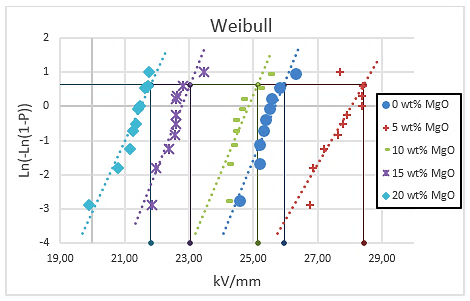
\includegraphics[width=0.55\textwidth]{image2.png}}{\fbox{Figure 1 Image}}
  \caption{Example of figure. (9 pt)}
  \label{fig:fig1}
\end{figure}

Example of table is shown in the following.

\begin{table}[htbp]
  \centering
  \caption{Example of table}
  \label{tab:tab1}
  \small
  \begin{tabular}{ccccc}
    \toprule
    \textbf{Variable (9pt)} & \textbf{Speed (rpm)} & \textbf{Power (kW)} & \textbf{Power (kW)} & \textbf{Power (kW)} \\
    \midrule
    (9 pt) a & 10 & 8.6  & 8.6  & 8.6  \\
    b        & 15 & 12.4 & 12.4 & 12.4 \\
    c        & 20 & 15.3 & 15.3 & 15.3 \\
    d        & 10 & 8.6  & 8.6  & 8.6  \\
    e        & 15 & 12.4 & 12.4 & 12.4 \\
    f        & 20 & 15.3 & 15.3 & 15.3 \\
    \bottomrule
  \end{tabular}
\end{table}

Example of combining multiple figure:

\begin{figure}[htbp]
  \centering
  \begin{subfigure}[b]{0.48\textwidth}
    \centering
    \IfFileExists{Gambar/image4.png}{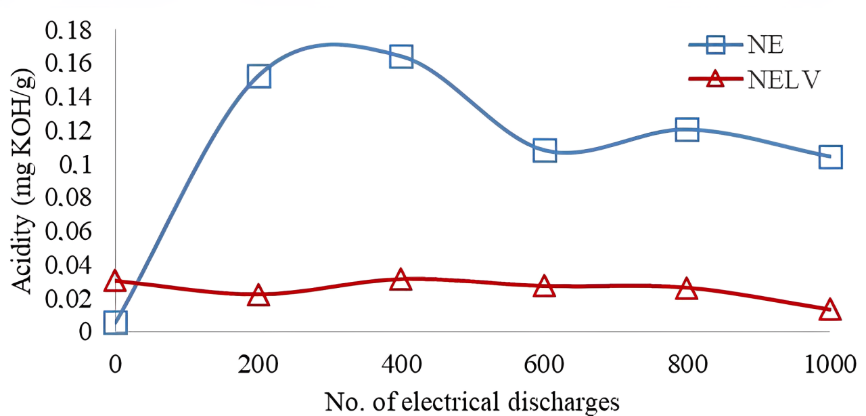
\includegraphics[width=\textwidth]{image4.png}}{\fbox{Figure 2(a)}}
    \caption{}
    \label{fig:fig2a}
  \end{subfigure}
  \hfill
  \begin{subfigure}[b]{0.48\textwidth}
    \centering
    \IfFileExists{Gambar/image5.jpg}{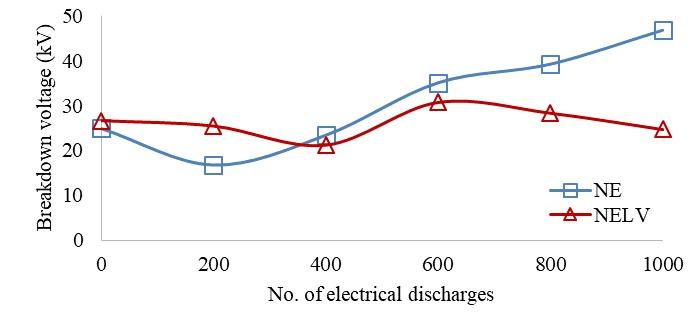
\includegraphics[width=\textwidth]{image5.jpg}}{\fbox{Figure 2(b)}}
    \caption{}
    \label{fig:fig2b}
  \end{subfigure}
  \caption{Example Effects of electrical discharges to (a) acidity of HVNE and NELV and (b) breakdown voltage of NE and NELV samples (9 pt)}
  \label{fig:fig2}
\end{figure}

% --- Section 3: Result and Discussions ---
\section{Result and Discussions (14 pt)}

In this section, it is explained the results of research and at the same time is given the comprehensive discussion. Results can be presented in figures, graphs, tables and others that make the reader understand easily \cite{sadowski2019data, saura2019comparing}. The discussion can be made in several sub-sections.

\subsection{Equations (12 pt)}

Equations should be placed at the center of the line and provided consecutively with equation numbers in parentheses flushed to the right margin, as in \eqref{eq:energy}. The use of Microsoft Equation Editor or MathType is preferred.

\begin{equation}
  E_v - E = \frac{\hbar^2}{2m} (k_x^2 + k_y^2)
  \label{eq:energy}
\end{equation}

All symbols that have been used in the equations should be defined in the following text.

\subsection{Algorithm or Pseudocode (12 pt)}

The algorithm or pseudocode is written using consolas font with 9 pt size and the alignment of the content is left. The name of the algorithm should be specified clearly. The description of the algorithm also should be stated in the require inside the table. See below example.

\begin{algorithm}[htbp]
\caption{Greedy search algorithm (10 pt)}
\label{alg:greedy}
\begin{algorithmic}[1]
\Require A graph $G(V,E)$, where $V$ is the set of vertices and $E$ is the set of edges; start node $s$; goal node $g$; heuristic function $h(n)$ that estimates the cost from any node $n$ to the goal.
\Ensure A path from start node $s$ to goal node $g$, if such a path exists.
\State Initialize $open\_list \gets [s]$
\State Initialize $came\_from \gets \text{empty map}$
\While{$open\_list$ is not empty}
    \State $current \gets \text{node in } open\_list \text{ with lowest } h(current)$
    \If{$current = g$}
        \State \Return $\text{ReconstructPath}(came\_from, current)$
    \EndIf
    \State remove $current$ from $open\_list$
    \For{each $neighbor$ in $\text{Neighbors}(current)$}
        \If{$neighbor$ not in $came\_from$}
            \State $came\_from[neighbor] \gets current$
            \State Add $neighbor$ to $open\_list$
        \EndIf
    \EndFor
\EndWhile
\State \Return \textbf{failure}
\end{algorithmic}
\end{algorithm}

\subsection{Citation (12 pt)}

Proper citation of other works should be made to avoid plagiarism. When referring to a reference item, please use the reference number as in \cite{nallaperuma2019online} or \cite{schulz2019advanced} for multiple references. The use of ``Ref \cite{shang2019data} \dots'' should be employed for any reference citation at the beginning of sentence. For any reference with more than 3 or more authors, only the first author is to be written followed by et al. (e.g. in \cite{yu2019clinical}). Examples of reference items of different categories shown in the References section. Each item in the references section should be typed using 8 pt font size \cite{huang2019queuing, xu2019internet, aqib2019smarter, leonelli2020data, stylos2019big, song2017tensor}.

\subsection{Level 3 Section 1 (10 pt)}

Lorem Ipsum is simply dummy text of the printing and typesetting industry. Lorem Ipsum has been the industry's standard dummy text ever since the 1500s, when an unknown printer took a galley of type and scrambled it to make a type specimen book.

\subsection{Level 3 Section 2 (10 pt)}

Lorem Ipsum is simply dummy text of the printing and typesetting industry. Lorem Ipsum has been the industry's standard dummy text ever since the 1500s, when an unknown printer took a galley of type and scrambled it to make a type specimen book.

% --- Section 4: Conclusion ---
\section{Conclusion (14 pt)}

Provide a statement that what is expected, as stated in the ``INTRODUCTION'' section can ultimately result in ``RESULTS AND DISCUSSION'' section, so there is compatibility. Moreover, the prospects for the development of research results and the application of further studies can also be added to the next (based on the results and discussion).

% --- Acknowledgements ---
\section*{Aknowledgements (If applicable) (12 pt)}

This section should acknowledge individuals who provided personal assistance to the work but do not meet the criteria for authorship, detailing their contributions. It is imperative to obtain consent from all individuals listed in the acknowledgments.

% --- References Guide & List ---
\section*{REFERENCES (12 pt)}

{\fontsize{8pt}{10pt}\selectfont
The main references are international journals and proceedings. All references should be to the most pertinent, up-to-date sources, and the minimum number of references should be 25 (for original research papers) and 50 (for review papers). References are written in IEEE style. You can access a more comprehensive guide at \url{http://ipmuonline.com/guide/refstyle.pdf}. Use a tool such as EndNote, Mendeley, or Zotero for reference management and formatting; choose IEEE style. Please use a consistent format for references---see examples (10 pt):\par}

\vspace{6pt}
{\fontsize{8.5pt}{11pt}\selectfont
\textbf{Journal/Periodicals}\\
\textit{Basic Format:}\\
J. K. Author, ``Title of paper,'' \textit{Abbrev. Title of Journal/Periodical}, vol. x, no. x, pp. xxx--xxx, Abbrev. Month, year, doi: xxx.\\
\textit{Examples:}\\
M. M. Chiampi and L. L. Zilberti, ``Induction of electric field in human bodies moving near MRI: An efficient BEM computational procedure,'' \textit{IEEE Trans. Biomed. Eng.}, vol. 58, pp. 2787--2793, Oct. 2011, doi: 10.1109/TBME.2011.2158315.\\
R. Fardel, M. Nagel, F. Nuesch, T. Lippert, and A. Wokaun, ``Fabrication of organic light emitting diode pixels by laser-assisted forward transfer,'' \textit{Appl. Phys. Lett.}, vol. 91, no. 6, Aug. 2007, Art. no. 061103, doi: 10.1063/1.2759475.
\par\vspace{4pt}

\textbf{Conference Proceedings}\\
\textit{Basic Format:}\\
J. K. Author, ``Title of paper,'' in \textit{Abbreviated Name of Conf.}, (location of conference is optional), year, pp. xxx--xxx, doi: xxx.\\
\textit{Examples:}\\
G. Veruggio, ``The EURON roboethics roadmap,'' in \textit{Proc. Humanoids '06: 6th IEEE-RAS Int. Conf. Humanoid Robots}, 2006, pp. 612--617, doi: 10.1109/ICHR.2006.321337.\\
J. Zhao, G. Sun, G. H. Loh, and Y. Xie, ``Energy-efficient GPU design with reconfigurable in-package graphics memory,'' in \textit{Proc. ACM/IEEE Int. Symp. Low Power Electron. Design (ISLPED)}, Jul. 2012, pp. 403--408, doi: 10.1145/2333660.2333752.
\par\vspace{4pt}

\textbf{Book}\\
\textit{Basic Format:}\\
J. K. Author, ``Title of chapter in the book,'' in \textit{Title of His Published Book}, X. Editor, Ed., xth ed. City of Publisher, State (only U.S.), Country: Abbrev. of Publisher, year, ch. x, sec. x, pp. xxx--xxx.\\
\textit{Examples:}\\
A. Taflove, \textit{Computational Electrodynamics: The Finite-Difference Time-Domain Method in Computational Electrodynamics II}, vol. 3, 2nd ed. Norwood, MA, USA: Artech House, 1996.\\
R. L. Myer, ``Parametric oscillators and nonlinear materials,'' in \textit{Nonlinear Optics}, vol. 4, P. G. Harper and B. S. Wherret, Eds., San Francisco, CA, USA: Academic, 1977, pp. 47--160.
\par\vspace{4pt}

\textbf{M. Theses (B.S., M.S.) and Dissertations (Ph.D.)}\\
\textit{Basic Format:}\\
J. K. Author, ``Title of thesis,'' M.S. thesis, Abbrev. Dept., Abbrev. Univ., City of Univ., Abbrev. State, year.\\
J. K. Author, ``Title of dissertation,'' Ph.D. dissertation, Abbrev. Dept., Abbrev. Univ., City of Univ., Abbrev. State, year.\\
\textit{Examples:}\\
J. O. Williams, ``Narrow-band analyzer,'' Ph.D. dissertation, Dept. Elect. Eng., Harvard Univ., Cambridge, MA, USA, 1993.\\
N. Kawasaki, ``Parametric study of thermal and chemical nonequilibrium nozzle flow,'' M.S. thesis, Dept. Electron. Eng., Osaka Univ., Osaka, Japan, 1993.
\par\vspace{4pt}

*In the reference list, however, list all the authors for up to six authors. Use et al. only if: 1) The names are not given and 2) List of authors more than 6. Example: J. D. Bellamy et al., \textit{Computer Telephony Integration}, New York: Wiley, 2010.
\par\vspace{4pt}
See the examples:
}

\vspace{6pt}
% Suppress extra thebibliography title to keep the single REFERENCES section header
\begingroup
\renewcommand{\section}[2]{}%
\begin{thebibliography}{99}
\fontsize{8pt}{10pt}\selectfont
\bibitem{sigala2019big}
M. Sigala, A. Beer, L. Hodgson, and A. O'Connor, \textit{Big Data for Measuring the Impact of Tourism Economic Development Programmes: A Process and Quality Criteria Framework for Using Big Data}. 2019.

\bibitem{nguyen2019machine}
G. Nguyen \textit{et al.}, ``Machine Learning and Deep Learning frameworks and libraries for large-scale data mining: a survey,'' \textit{Artif. Intell. Rev.}, vol. 52, no. 1, pp. 77--124, 2019, doi: 10.1007/s10462-018-09679-z.

\bibitem{shorten2019survey}
C. Shorten and T. M. Khoshgoftaar, ``A survey on Image Data Augmentation for Deep Learning,'' \textit{J. Big Data}, vol. 6, no. 1, 2019, doi: 10.1186/s40537-019-0197-0.

\bibitem{vinayakumar2019deep}
R. Vinayakumar, M. Alazab, K. P. Soman, P. Poornachandran, A. Al-Nemrat, and S. Venkatraman, ``Deep Learning Approach for Intelligent Intrusion Detection System,'' \textit{IEEE Access}, vol. 7, pp. 41525--41550, 2019, doi: 10.1109/ACCESS.2019.2895334.

\bibitem{sivaraman2019network}
K. Sivaraman, R. M. V. Krishnan, B. Sundarraj, and S. Sri Gowthem, ``Network failure detection and diagnosis by analyzing syslog and SNS data: Applying big data analysis to network operations,'' \textit{Int. J. Innov. Technol. Explor. Eng.}, vol. 8, no. 9 Special Issue 3, pp. 883--887, 2019, doi: 10.35940/ijitee.I3187.0789S319.

\bibitem{dwivedi2019decentralized}
A. D. Dwivedi, G. Srivastava, S. Dhar, and R. Singh, ``A decentralized privacy-preserving healthcare blockchain for IoT,'' \textit{Sensors (Switzerland)}, vol. 19, no. 2, pp. 1--17, 2019, doi: 10.3390/s19020326.

\bibitem{alturjman2019quantifying}
F. Al-Turjman, H. Zahmatkesh, and L. Mostarda, ``Quantifying uncertainty in internet of medical things and big-data services using intelligence and deep learning,'' \textit{IEEE Access}, vol. 7, pp. 115749--115759, 2019, doi: 10.1109/ACCESS.2019.2931637.

\bibitem{kumar2019big}
S. Kumar and M. Singh, ``Big data analytics for healthcare industry: Impact, applications, and tools,'' \textit{Big Data Min. Anal.}, vol. 2, no. 1, pp. 48--57, 2019, doi: 10.26599/BDMA.2018.9020031.

\bibitem{ang2019deployment}
L. M. Ang, K. P. Seng, G. K. Ijemaru, and A. M. Zungeru, ``Deployment of IoV for Smart Cities: Applications, Architecture, and Challenges,'' \textit{IEEE Access}, vol. 7, pp. 6473--6492, 2019, doi: 10.1109/ACCESS.2018.2887076.

\bibitem{lau2019survey}
B. P. L. Lau \textit{et al.}, ``A survey of data fusion in smart city applications,'' \textit{Inf. Fusion}, vol. 52, no. January, pp. 357--374, 2019, doi: 10.1016/j.inffus.2019.05.004.

\bibitem{wu2019large}
Y. Wu \textit{et al.}, ``Large scale incremental learning,'' \textit{Proc. IEEE Comput. Soc. Conf. Comput. Vis. Pattern Recognit.}, vol. 2019-June, pp. 374--382, 2019, doi: 10.1109/CVPR.2019.00046.

\bibitem{mosavi2019prediction}
A. Mosavi, S. Shamshirband, E. Salwana, K. wing Chau, and J. H. M. Tah, ``Prediction of multi-inputs bubble column reactor using a novel hybrid model of computational fluid dynamics and machine learning,'' \textit{Eng. Appl. Comput. Fluid Mech.}, vol. 13, no. 1, pp. 482--492, 2019, doi: 10.1080/19942060.2019.1613448.

\bibitem{palanisamy2019implications}
V. Palanisamy and R. Thirunavukarasu, ``Implications of big data analytics in developing healthcare frameworks --- A review,'' \textit{J. King Saud Univ. - Comput. Inf. Sci.}, vol. 31, no. 4, pp. 415--425, 2019, doi: 10.1016/j.jksuci.2017.12.007.

\bibitem{sadowski2019data}
J. Sadowski, ``When data is capital: Datafication, accumulation, and extraction,'' \textit{Big Data Soc.}, vol. 6, no. 1, pp. 1--12, 2019, doi: 10.1177/2053951718820549.

\bibitem{saura2019comparing}
J. R. Saura, B. R. Herraez, and A. Reyes-Menendez, ``Comparing a traditional approach for financial brand communication analysis with a big data analytics technique,'' \textit{IEEE Access}, vol. 7, pp. 37100--37108, 2019, doi: 10.1109/ACCESS.2019.2905301.

\bibitem{nallaperuma2019online}
D. Nallaperuma \textit{et al.}, ``Online Incremental Machine Learning Platform for Big Data-Driven Smart Traffic Management,'' \textit{IEEE Trans. Intell. Transp. Syst.}, vol. 20, no. 12, pp. 4679--4690, 2019, doi: 10.1109/TITS.2019.2924883.

\bibitem{schulz2019advanced}
S. Schulz, M. Becker, M. R. Groseclose, S. Schadt, and C. Hopf, ``Advanced MALDI mass spectrometry imaging in pharmaceutical research and drug development,'' \textit{Curr. Opin. Biotechnol.}, vol. 55, pp. 51--59, 2019, doi: 10.1016/j.copbio.2018.08.003.

\bibitem{shang2019data}
C. Shang and F. You, ``Data Analytics and Machine Learning for Smart Process Manufacturing: Recent Advances and Perspectives in the Big Data Era,'' \textit{Engineering}, vol. 5, no. 6, pp. 1010--1016, 2019, doi: 10.1016/j.eng.2019.01.019.

\bibitem{yu2019clinical}
Y. Yu, M. Li, L. Liu, Y. Li, and J. Wang, ``Clinical big data and deep learning: Applications, challenges, and future outlooks,'' \textit{Big Data Min. Anal.}, vol. 2, no. 4, pp. 288--305, 2019, doi: 10.26599/BDMA.2019.9020007.

\bibitem{huang2019queuing}
M. Huang, W. Liu, T. Wang, H. Song, X. Li, and A. Liu, ``A queuing delay utilization scheme for on-path service aggregation in services-oriented computing networks,'' \textit{IEEE Access}, vol. 7, pp. 23816--23833, 2019, doi: 10.1109/ACCESS.2019.2899402.

\bibitem{xu2019internet}
G. Xu, Y. Shi, X. Sun, and W. Shen, ``Internet of things in marine environment monitoring: A review,'' \textit{Sensors (Switzerland)}, vol. 19, no. 7, pp. 1--21, 2019, doi: 10.3390/s19071711.

\bibitem{aqib2019smarter}
M. Aqib, R. Mehmood, A. Alzahrani, I. Katib, A. Albeshri, and S. M. Altowaijri, \textit{Smarter traffic prediction using big data, in-memory computing, deep learning and gpus}, vol. 19, no. 9. 2019.

\bibitem{leonelli2020data}
S. Leonelli and N. Tempini, \textit{Data Journeys in the Sciences}. 2020.

\bibitem{stylos2019big}
N. Stylos and J. Zwiegelaar, \textit{Big Data as a Game Changer: How Does It Shape Business Intelligence Within a Tourism and Hospitality Industry Context?} 2019.

\bibitem{song2017tensor}
Q. Song, H. Ge, J. Caverlee, and X. Hu, ``Tensor completion algorithms in big data analytics,'' \textit{arXiv}, vol. 13, no. 1, 2017.
\end{thebibliography}
\endgroup

\end{document}
